\section{Non-Dim of NS}
\begin{gather*}
    t^* = ft, \; \vec{x}^* = \frac{\vec{x}}{L}, \; v^* = \frac{\vec{v}}{V} \\
    P^* \frac{P - P_\infty}{P_0 - P_\infty}, \; g^* = \frac{\vec{g}}{g}, \; \vec{\nabla}^* = L \vec{\nabla} 
\end{gather*}
Non-dimensionalized NS:
\begin{align*}
    [\text{St}] \frac{\partial v^*}{\partial t^*} &+ (\vec{v} \cdot \vec{\nabla})\vec{v}^* = - [\text{Eu}] \vec{\nabla} P^*  \\
    & \; + [\text{Fr}^{-2}] \vec{g}^* + [\text{Re}^{-1}] \vec{\nabla}^2 \vec{v}^* 
\end{align*}
where
\begin{align*}
    \text{St} &= \frac{fL}{V}, \; \text{Eu} = \frac{P_0 - P_\infty}{\rho V^2} \\
    \text{Fr} &= \frac{V^2}{gL}, \; \text{Re} = \frac{\rho V L}{\mu}
\end{align*}
\subsection{Creeping Flow (Stokes Flow)}
Re $\ll 1$, viscous forces dominate, inertia negligible. NS becomes:
\begin{align*}
    \vec{\nabla} P &= \mu \vec{\nabla}^2 \vec{v} 
\end{align*}
Drag on creeping flow,
\begin{align*}
    F_D &= c V L \mu, \; F_{D, \text{sphere}} = 3 \pi \mu V D
\end{align*}
Typical balance for falling sphere:
\begin{align*}
    W &= F_D + F_\text{buoyancy}
\end{align*}
\begin{align*}
    F_\text{buoyancy} &= \frac{\pi D^3}{6} \rho_{\text{fluid}} g, \; W = \rho_{\text{particle}} \frac{\pi D^3}{6} g
\end{align*}
\subsection{Inviscid Flow (Euler Flow)}
Viscous stresses are negligible, $\tau \approx 0$. Typically high Re, away from wall. Can't specify no-slip at wall. 
\begin{align*}
    \rho \left[\frac{\partial \vec{v}}{\partial t} + (\vec{v} \cdot \vec{\nabla})\vec{v}\right] &= -\vec{\nabla} P + \rho \vec{g}
\end{align*}
a consequence, 
\begin{align*}
    \frac{P}{\rho} + \frac{V^2}{2} + gz &= \text{constant along streamline}
\end{align*}
Check shear to make sure 0:
\begin{align*}
    \tau &= \mu \frac{\partial U}{\partial y} \\
    \tau_{r \theta} &= \mu \left(r \frac{\partial}{\partial r} \left(\frac{u_\theta}{r}\right) + \frac{1}{r} \frac{\partial u_r}{\partial \theta}\right)
\end{align*}
\subsection{Irrotational Flow}
$\vec{\nabla} \times \vec{v} = 0$. Velocity potential, $\phi$,
\begin{gather*}
    u = \frac{\partial \phi}{\partial x}, \; v = \frac{\partial \phi}{\partial y}, \; w = \frac{\partial \phi}{\partial z} \\
    u_r = \frac{\partial \phi}{\partial r}, \; u_\theta = \frac{1}{r} \frac{\partial \phi}{\partial \theta}, \; u_z = \frac{\partial \phi}{\partial z}
\end{gather*}
Solve cont. ($\nabla^2 \phi = 0$), calculate $\vec{v}$, and calculate P from Bernoulli. Bernoulli is \textbf{constant everywhere} for irrotational flow.
\begin{align*}
    \nabla^2 \phi &= \frac{\partial^2 \phi}{\partial x^2} + \frac{\partial^2 \phi}{\partial y^2} + \frac{\partial^2 \phi}{\partial z^2} = 0\\
    \nabla^2 \phi &= \frac{1}{r} \frac{\partial}{\partial r} \left(r \frac{\partial \phi}{\partial r}\right) + \frac{1}{r^2} \frac{\partial^2 \phi}{\partial \theta^2} + \frac{\partial^2 \phi}{\partial z^2} = 0
\end{align*}
\section{Boundary Layer}
Laminar BL assumptions are: steady, incomp, 2D, Re is large such that $\delta/x \ll 1$, BL stays laminar:
\begin{align*}
    u \frac{\partial u}{\partial x} + v \frac{\partial u}{\partial y} &= \nu \frac{\partial^2 u}{\partial y^2} \\
    \frac{\partial u}{\partial x} + \frac{\partial v}{\partial y} &= 0
\end{align*}
Blasius similarity variable
\begin{align*}
    \eta = y \sqrt{\frac{U_\infty}{\nu x}}, \; f' = \frac{f}{U_\infty}
\end{align*}
Blasius solution for flat plate:
\vspace{-10pt}
\begin{table}[H]
    \centering
    \footnotesize
    \resizebox{0.24\textwidth}{!}{
    \begin{tabular}{p{0.06\textwidth}cc}
        \toprule
        & Laminar & Turbulent \\
        \midrule
        BL Thick. & $\frac{\delta}{x} = \frac{4.91}{\sqrt{\text{Re}_x}}$ & $\frac{\delta}{x} = \frac{0.16}{(\text{Re}_x)^{1/7}}$ \\
        Displ. Thick. & $\frac{\delta^*}{x} = \frac{1.72}{\sqrt{\text{Re}_x}}$ & $\frac{\delta^*}{x} = \frac{0.20}{(\text{Re}_x)^{1/7}}$ \\
        Momen. Thick. & $\frac{\theta}{x} = \frac{0.664}{\sqrt{\text{Re}_x}}$ & $\frac{\theta}{x} = \frac{0.016}{(\text{Re}_x)^{1/7}}$ \\
        Local Skin Fric. Coeff. & $C_{f, x} = \frac{0.664}{\sqrt{\text{Re}_x}}$ & $C_{f, x} = \frac{0.027}{\text{Re}_x^{1/7}}$ \\
        % $\frac{\delta}{x} = \frac{4.91}{\sqrt{\text{Re}_x}}$ & $\frac{\delta}{x} = \frac{0.16}{(\text{Re}_x)^{1/7}}$ \\
        % $\frac{\delta^*}{x} = \frac{1.72}{\sqrt{\text{Re}_x}}$ & $\frac{\delta^*}{x} = \frac{0.20}{(\text{Re}_x)^{1/7}}$ \\
        % $\frac{\theta}{x} = \frac{0.664}{\sqrt{\text{Re}_x}}$ & $\frac{\theta}{x} = \frac{0.016}{(\text{Re}_x)^{1/7}}$ \\
        % $C_{f, x} = \frac{0.664}{\sqrt{\text{Re}_x}}$ & $C_{f, x} = \frac{0.027}{\text{Re}_x^{1/7}}$ \\
        \bottomrule
    \end{tabular}
    } \vspace{-20pt}
\end{table}
Displacement thickness
\begin{align*}
    \delta^* = \int_0^\delta (1 - \frac{u}{U_\infty}) \, dy
\end{align*}
Momentum thickness
\begin{align*}
    \theta = \int_0^\delta \frac{u}{U_\infty} (1 - \frac{u}{U_\infty}) \, dy
\end{align*}
Drag Coefficient
\begin{align*}
    C_D = \frac{2 F_D}{\rho V^2 A}
\end{align*}
\subsection{1D Isentropic Nozzle}
Assumptions: 1D (negligible boundary layer effects); steady; adiabatic; ideal gas; isentropic; inlet conditions do not change appreciably.
Stagnation properties:
\begin{align*}
    h_0 &= h + \frac{V^2}{2} \\
    T_0 &= T+ \frac{V^2}{2 c_p} 
\end{align*}
If isentropic:
\begin{align*}
    \frac{P_0}{P} &= \left(\frac{T_0}{T}\right)^{\frac{k}{k-1}} \\
    \frac{\rho_0}{\rho} &= \left(\frac{T_0}{T}\right)^{\frac{1}{k-1}}
\end{align*}
Speed of sound:
\begin{align*}
    c &= \sqrt{\left(\frac{\partial P}{\partial \rho}\right)_s} = \sqrt{k R T}
\end{align*}
Mach number:
\begin{align*}
    \text{Ma} &= \frac{V}{c}
\end{align*}
For an expansion with $\uparrow A$:
\vspace{-15pt}
\begin{table}[H]
    \centering
    \footnotesize
    \begin{tabular}{cc}
        \toprule
        Subsonic & Supersonic \\
        \midrule
        $\downarrow V, \text{Ma}$ & $\uparrow V, \text{Ma}$ \\
        $\downarrow P, \rho$ & $\uparrow P, \rho$ \\
        \bottomrule
    \end{tabular}
\end{table} \vspace{-25pt}
And if $c_p$ is constant:
\begin{align*}
    \frac{T_0}{T} &= 1 + \frac{k-1}{2} \text{Ma}^2 \\
    \frac{P_0}{P} &= \left(1 + \frac{k-1}{2} \text{Ma}^2\right)^{\frac{k}{k-1}} \\
    &= \frac{\rho_0}{\rho}
\end{align*}
When Ma$=1$ (at throat), critical properties are 
\begin{align*}
    \frac{T^*}{T_0} &= \frac{2}{k+1} \\
    \frac{P^*}{P_0} &= \left(\frac{2}{k+1}\right)^{\frac{k}{k-1}} \\
    &= \frac{\rho^*}{\rho_0}
\end{align*}
so exit pressure:
\begin{align*}
    P_e &= \begin{cases}
        P_b, & P_b > P^* (\text{subsonic}, \text{Ma}<1) \\
        P^*, & P_b \leq P^* (\text{sonic/chocked}, \text{Ma}=1) \\
    \end{cases}
\end{align*}
mass flow:
\begin{align*}
    \dot{m} &= \rho A V \\
    &= P_0 A \text{Ma} \sqrt{\frac{k}{R T_0}}\left(1 + \frac{k-1}{2} \text{Ma}^2\right)^{\frac{-k-1}{2(k-1)}} \\
    \dot{m}_\text{max} &= P_0 A^* \sqrt{\frac{k}{R T_0}}\left(\frac{2}{k+1}\right)^{\frac{k+1}{2(k-1)}} \\
    &= \rho^* A^* V^*
\end{align*}
note, max mass flow is when Ma$=1$ and $A = A^*$. For converging-diverging nozzles,
\begin{align*}
    \frac{A}{A^*} &= \frac{1}{\text{Ma}}\left(\frac{2}{k+1}\cdot \left(1 + \frac{k-1}{2}\right)\right)^{\frac{k+1}{2(k-1)}}
\end{align*}
% \begin{figure}[H]
%     \centering
%     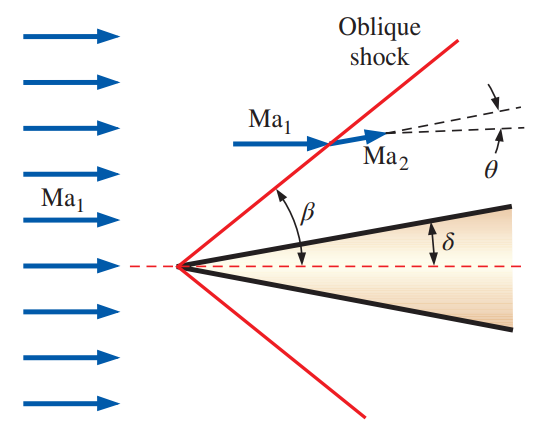
\includegraphics[width=0.13\textwidth]{Figures/oblique.png}
%     \caption*{Oblique Shock}
% \end{figure} \vspace{-20pt}
% \begin{figure}[H]
%     \centering
%     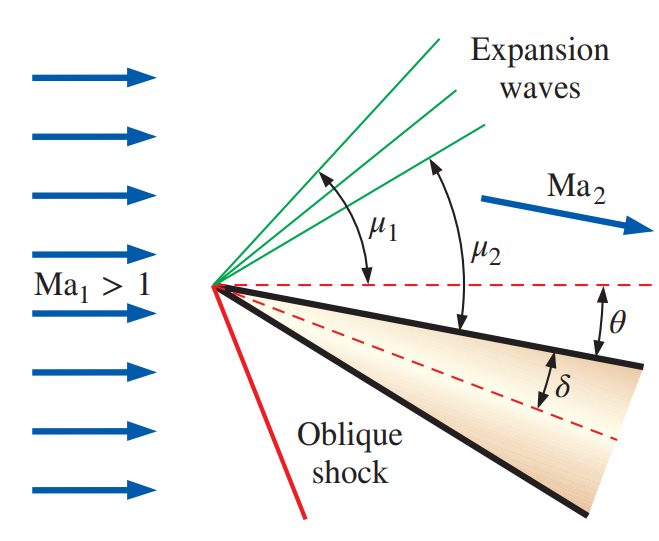
\includegraphics[width=0.13\textwidth]{Figures/expansion fan.png}
%     \caption*{Expansion Fan}
% \end{figure}
\begin{figure}[H]
    \centering
    \begin{minipage}{0.11\textwidth}
        \centering
        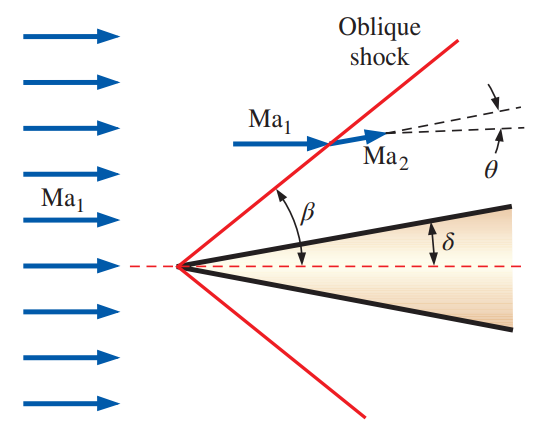
\includegraphics[width=0.8\textwidth]{Figures/oblique.png}
        \caption*{Oblique Shock}
    \end{minipage}
    \begin{minipage}{0.11\textwidth}
        \centering
        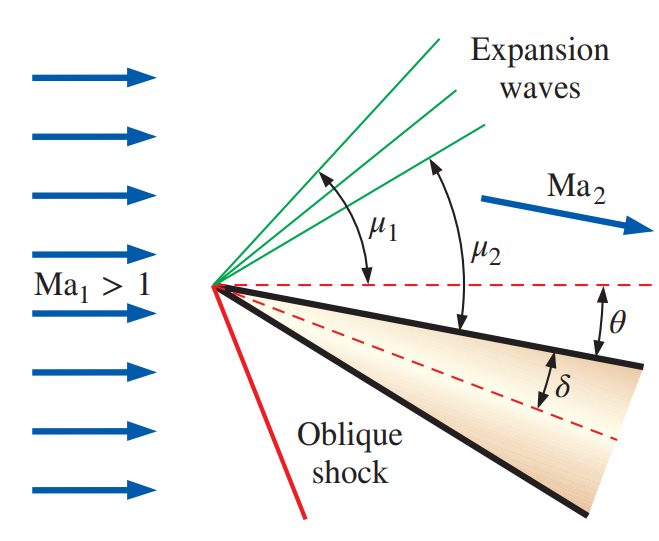
\includegraphics[width=0.8\textwidth]{Figures/expansion fan.png}
        \caption*{Expansion Fan}
    \end{minipage}
\end{figure}
\subsection{Normal Shock}
Region 1 is upstream, Region 2 is downstream. The shock is not isentropic. 
\begin{align*}
    T_{01} &= T_{02} \\
    \text{Ma}_2 &= \sqrt{\frac{(k - 1)\text{Ma}_1^2 + 2}{2k\text{Ma}_1^2 - (k-1)}} \\
    \frac{P_2}{P_1} &= \frac{2k\text{Ma}_1^2 - (k-1)}{k+1} \\
    \frac{\rho_2}{\rho_1} &= \frac{P_2/P_1}{T_2/T_1} = \frac{(k+1)\text{Ma}_1^2}{2 + (k-1)\text{Ma}_1^2} = \frac{V_1}{V_2} \\
    \frac{T_2}{T_1} &= \frac{2 + \text{Ma}_1^2(k-1)}{2 + \text{Ma}_2^2(k-1)} \\
    \frac{P_{02}}{P_{01}} &= \frac{\text{Ma}_1}{\text{Ma}_2} \left(\frac{1 + \text{Ma}_1^2(k-1)/2}{1 + \text{Ma}_2^2(k-1)/2}\right)^{\frac{k+1}{2(k-1)}} \\
    s_2 - s_1 &= c_p \ln\left(\frac{T_2}{T_1}\right) - R \ln\left(\frac{P_2}{P_1}\right) \\
\end{align*}

\subsection{Oblique Shock}
$\theta$ is the turning angle, $\beta$ is the shock angle. \textbf{If thin boundary layer}, $\delta = \theta$.
 %\vspace{-10pt}
The \textbf{normal components} of the shock is the \textbf{same} as a \textbf{normal shock}. Use $\text{Ma}_{n}$ and $V_{n}$ for normal components. Pressure, temperature, and density are still $P_0, T_0, \rho_0$.
The normal components:
\begin{align*}
    \text{Ma}_{1, n} &= \text{Ma}_1 \sin\beta \\
    \text{Ma}_{2, n} &= \text{Ma}_2 \sin(\beta - \theta)
\end{align*}
\begin{align*}
    \tan\theta &= \frac{2\cot\beta (\text{Ma}_1^2 \sin^2\beta - 1)}{\text{Ma}_1^2 (k + \cos 2\beta) + 2} 
\end{align*}
Mach angle,
\begin{align*}
    \mu &= \sin^{-1}\left(1/\text{Ma}_1\right)
\end{align*}

\subsection{Expansion Waves}
\begin{align*}
    \theta &= \nu(\text{Ma}_2) - \nu(\text{Ma}_1) \\
    \nu(\text{Ma}) &= \sqrt{\frac{k + 1}{k - 1}} \tan^{-1} \sqrt{\frac{k - 1}{k + 1}(\text{Ma}^2 - 1)} \\
    & \quad - \tan^{-1}\sqrt{\text{Ma}^2 - 1}
\end{align*}
Use isentropic relations to find properties across the wave.